\subsection{Influence of trend}
\label{sec:influenceOfTrendInCalcInput}
Calculated inputs showed very different results. The electricity price prediction showed an overall improvement when adding slope, skewness and volatility as input. The alternative scatter approach from \cite{singhal2011electricity} where previous hours are directly added as inputs for the network to calculate the relationship itself was outperformed by the direct input calculations. Skewness and volatility obtained the best result for prices with an improvement of 4\% compared to the prediction without these inputs. The results for wind power was different since only one of the calculated inputs, volatility, showed an improvement of 3,52\% compared to the same prediction without that input. It was established in the analysis that both price and wind power are highly volatile and consists of different types of spikes during the year. The need for including characteristics about these spikes are discussed in Section~\ref{sec:usingStatisticalInput} but in brief it is related to the current price behaviour reflecting current market conditions and by including a calculation thereof we hope to add more characteristics of the output we are trying to predict. 

We also conducted an experiment on the simplest electricity price dataset consisting of last-known price and demand where we tested the impacts of the calculated inputs. This test compared to the one without calculated inputs showed an improvement of 21,24\% in the favour of the calculated inputs. This strengthens that the calculated inputs improve the predictions and that other statistical methods might improve it further. The need for adapting to changes in trends and seasons are also presented in \cite{forecastingSpotPricesAccountingForWindPower}. It is the only text included that also attempts to predict the day-ahead spot prices from Nord Pool Spot for Western Denmark. They use a simple regression model and more sophisticated two-step models to capture and adapt to seasonal changes and shifts in trends. The specific models from \cite{forecastingSpotPricesAccountingForWindPower} are Holt-Winters in two variations, ARIMAX and a seasonal persistence model --- we wont go into greater detail with other than the purpose of them is to capture seasonal changes and trends. Since they are predicting the exact same market and use the same electricity prices from Nord Pool Spot we use it to exemplify other achievements of electricity price prediction within the same market. It stands in contrast to the discussion regarding comparison of neural networks in different markets --- but this is the same market, the same currency and the exact same data format we are trying to predict. Furthermore their training dataset covers more than a year of unseen data from 2009-2011. The comparison is not one-to-one since they use older data than ours but it can give an indication of where we position ourselves. Table~\ref{table:resultComparisonWithOtherDanishText} shows that their results vary from 33,66 to 69,75. We position ourselves better than their standard persistence model but obtain close numbers to ARIMA and standard Holt-Winters. Their two-step Holt-Winter model significantly outperforms all others and show the room for improvements and future work of our approach. The text mentions that a model that might be just as suitable as theirs are an Adaptive Wavelet Neural Network. This has not been considered in this thesis but investigations can be made in future work. Their Holt-Winter approach verifies our initial thoughts from Section~\ref{sec:usingStatisticalInput} about how important it is to analyse seasonal changes and trend shifts to further characterise the output to predict. Their approach does not include the trend as calculated inputs because there is a potential for not being able to generalize over all the different trends in the dataset (remember that we calculate trend for a predefined number of previous hours for all hours in the dataset which is what we try to generalize upon). 

\footnotesize
\begin{center}
\begin{longtable}{|c|c|}
\hline
\textbf{Model} & \textbf{MAE (DKK)} \\
\hline
\endfirsthead
\multicolumn{2}{c}%
{\tablename\ \thetable\ -- \textit{Continued from previous page}} \\
\hline
\textbf{Model} & \textbf{MAE (DKK)}  \\
\hline
\endhead
\hline \multicolumn{2}{r}{\textit{Continued on next page}} \\
\endfoot
\hline
\endlastfoot
\arrayrulecolor{light-gray}
Two-step Holt-Winters & 33,66\\ \hline
Holt-Winters & 40,34 \\ \hline
ARIMAX & 43,26 \\ \hline
Our ANN model & 45,17 \\ \hline
Seasonal persistence model & 69,75 \\ \hline
\caption{Results from various prediction models on unseen data.}
\label{table:resultComparisonWithOtherDanishText}
\end{longtable}
\end{center}
\normalsize

\subsubsection{Calculated Inputs}
Using inputs that analyse on a predefined number of previous hours for every hour of the dataset (except from the first hours without enough previous hours) can have both positive and negative results depending on what to predict as seen in our experiments. The purpose is to get a more precise prediction from step to step in the 24-step-ahead prediction. The potential of elevating the error arises if the first steps are inaccurate because it will have an effect on some of the the following steps. This is reflected in slope calculation as input for wind power in Section~\ref{sec:windPowerSlopeCalc} and seen in the comparison without it in Figure~\ref{fig:basicCurveAnalysisGraphoForDiscussion} --- this will be elaborated in the coming section about step ahead prediction in Section~\ref{sec:stepAheadDiscussion}. 

It is noticeable that the same calculations do not apply for both price and wind power even though they possess similar characteristics. It is therefore necessary to experiment thoroughly with the different approaches in order to find the most applicable for a specific dataset --- this emphasizes the discussion from the input parameters Section~\ref{sec:inputParameterDiscussion} regarding the need for describing and analysing the dataset because what worked for one dataset does not necessarily work for others if the two datasets are completely different. The calculated inputs are based on prices and productions from previous hours and because markets are different it must be stated clearly what factors are used. For instance, countries with many Cooling Degree Days or Heating Degree Days (following the model in Section~\ref{sec:ElectricityDemand}) have higher consumption which greatly influence the price and its behaviour. The same apply for the importance of wind power in the Danish electricity market due to the large amount of wind mills which in this thesis has shown to be significant. This is most likely not applicable for countries without the same amount of mills. The documentation is a contributory factor to the potential of identifying similar markets in terms of influences. It can help identify both standard and calculated inputs for specific market conditions, e.g. if a market is analysed to be similar to Denmark then it makes sense to use their ideas and models first and build from them if they perform well.

\begin{figure}[H]
\centering
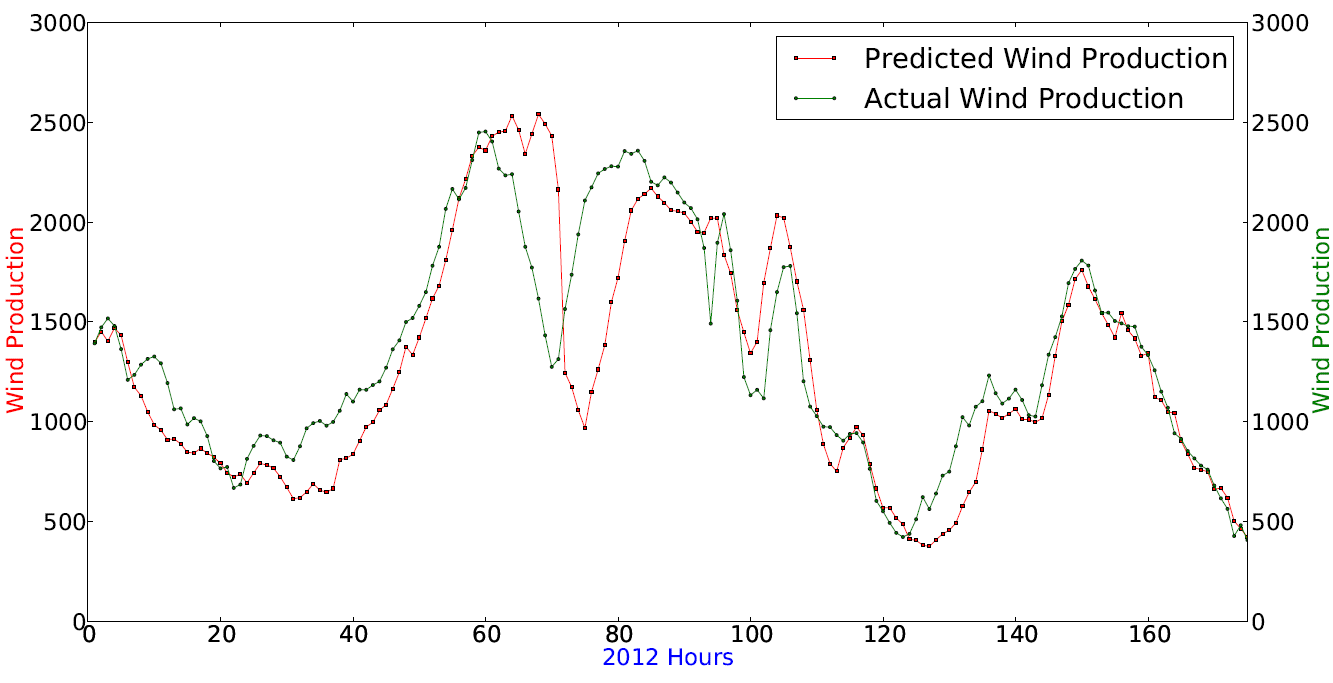
\includegraphics[width=0.99\linewidth]{billeder/curveAnalysisWindProduction.png}
\caption{Wind production prediction for 175 hours in 2012 with slope as input}
\label{fig:basicCurveAnalysisGraphoForDiscussion}
\end{figure}

It was expected to see better accuracy when applying calculated inputs to the electricity prices since it relies more heavily on previous prices and price movements in general as discussed in the price analysis in Section~\ref{sec:ElectricityPriceAnalysis}. Wind power follows meteorological factors more significantly which is expressed in the correlation to wind speed. The problem can be related to the electricity price being extremely volatile and the network not being able to identify a general recognizable pattern in how immediate hours impact the electricity prices when calculated (mentioned in Section~\ref{sec:usingStatisticalInput}).

The analysis establishes that previous hours impact the price and wind power but not if the actual skewness or historical volatility calculations have an influence. The reason is the many adjustable settings (see Section~\ref{sec:windProductionDev}) of the functions which in our opinion makes them more applicable for testing directly in experiments based on the conclusion that previous hours influence the output. What can be concluded from the results is the potential benefit from using calculated inputs to add additional characteristics about the movements of the curve and help the generalization function of the network to approach its target better --- if the correct calculated inputs are used. Alternative calculations from the field of economics could be investigated to include additional features and characteristics of the curve movements but also hybrid versions of the Feedforward Neural Network can be studied. One such hybrid is a Wavelet Neural Network (WNN) where the properties of a wavelet is utilized in \cite{adaptiveWaveletANNElectricityMarkets} and the wavelet shape is adapted according to the training dataset instead of adapting the parameters of a fixed shape function (an example is the sigmoid function) by adjusting weights. Their point is that a WNN is better at generalizing high frequency signals than the Feedforward Neural Network that we are using here. It has not been considered in this thesis but based on the above description it potentially can improve the accuracy.